\documentclass[12pt,letterpaper]{article}

\author{Jacob Thomas Errington}
\date{15 February 2017}
\title{Assignment \#2\\Discrete structures 2 -- MATH 340}

\usepackage[margin=2.0cm]{geometry}
\usepackage{amsmath,amssymb,amsthm}
\usepackage{tikz}

\usetikzlibrary{graphs}

%%%%% Set up sections to be questions

\renewcommand{\thesection}{Question \arabic{section}}
\newcommand{\question}{\section}

%%%%% Set up math notations

\newtheorem{prop}{Proposition}
\DeclareMathOperator{\degOp}{deg}
\newcommand{\parens}[1]{\left(#1\right)}
\renewcommand{\deg}[1]{\degOp{\parens{#1}}}
\DeclareMathOperator{\chromOp}{\chi}
\newcommand{\chrom}[1]{\chromOp{\parens{#1}}}
\newcommand{\half}{\frac{1}{2}}
\newcommand{\degrees}{^\circ}
\newcommand{\mknode}[1]{\node[mynode] (#1) {} ;}

\tikzset{
    mynode/.style={
        inner sep=0,
        draw,
        circle,
        fill=black!15,
        minimum width=1em,
    },
    nice graph/.style={
        row sep=1em,
        column sep=1em,
    },
}

\begin{document}

\maketitle

\question{Euler's formula}

\begin{prop}
    Suppose $G$ is a planar graph such that every vertex in $G$ has degree at
    least five, and at least one vertex in $G$ has degree eight.
    Then, $G$ has at least 15 vertices.
\end{prop}

\begin{proof}
    Let $n = |V(G)|$ and $e = |E(G)|$.
    From Euler's formula we have the upper bound on the number of edges
    \begin{equation}
        \label{eq:euler-lower-bound}
        3n - 6 \geq e
    \end{equation}
    From the assumptions, we know that every vertex has degree at least five,
    so by the handshaking lemma
    \begin{equation}
        \label{eq:handshake-lower-bound}
        \sum_{v \in V(G)} \deg{v} = 2 e \geq 5 n
    \end{equation}
    However, we also know that at least one vertex has degree eight, so the
    lower bound in \eqref{eq:handshake-lower-bound} on the edges can be bumped
    up by three, giving
    \begin{equation}
        \label{eq:shake-better-lower-bound}
        2 e \geq 5 n + 3
    \end{equation}
    We combine the bounds in \eqref{eq:shake-better-lower-bound} and
    \eqref{eq:euler-lower-bound} by transitivity to obtain
    \begin{equation*}
        2(3n - 6) \geq 5n + 3
    \end{equation*}
    Some algebraic manipulation gives the desired bound $n \geq 15$.
\end{proof}

\begin{prop}
    Suppose $G$ is a triangulation of the plane. Then, the number of faces of
    $G$ is even.
\end{prop}

\begin{proof}
    Since every face in a triangulation is bounded by exactly three edges, we
    get the following relation between the number of faces and the number of
    edges.
    \begin{equation*}
        \label{eq:tri-face-edge-rel}
        2 |E| = 3 |F|
    \end{equation*}
    Using this relation, we can eliminate $E$ in Euler's formula to get.
    \begin{equation*}
        |V| - \frac{3}{2} |F| + |F| = 2
    \end{equation*}
    Algebraic manipulation gives $|F| = 2|V| - 4$, which is even for any size
    of $V$.
\end{proof}

\question{Coloring planar graphs}

\begin{prop}
    Suppose that a planar graph $G = (V, E)$ has no $K_3$ subgraph.
    Then, $\chrom{G} \leq 4$.
\end{prop}

\begin{proof}
    Not having a $K_3$ subgraph means that the graph contains no triangles, or
    cycles of length three. Hence, every face in $G$ is bounded by at least $4$
    edges.

    Suppose that every face in $G$ were bounded by \emph{exactly} four edges.
    Then $4|F| = 2|E|$.
    Substituting into Euler's formula gives $|V| - |E| + \half |E| = 2$, which
    can be rewritten as $2|V| - 4 = |E|$. However, our graph does not have each
    face bounded by \emph{exactly} four edges, but rather by \emph{at least}
    four edges, which gives us an upper bound on the number of edges.
    \begin{equation}
        \label{eq:edge-upper-bound}
        2|V| - 4 \geq |E|
    \end{equation}

    Combining this bound with the handshaking lemma gives
    \begin{equation}
        \label{eq:bounded-handshake}
        \sum_{v \in V} \deg{v} = 2 |E| \leq 4 |V| - 8 < 4 |V|
    \end{equation}

    This shows that the average degree is less strictly less than $4$, so there
    must be an edge with degree at most $3$.

    This shows that $G$ is $3$-degenerate. (Take any subgraph of $G$. It also
    has no $K_3$ subgraph. Hence the above argument applies to it as well.)
    Thus by a theorem, $\chrom{G} \leq 4$.
\end{proof}

The following proposition is \emph{false.}

\begin{prop}
    If a planar graph has no $K_4$ subgraph, then $\chrom{G} \leq 3$.
\end{prop}

To see that the proposition is false, consider the graph in figure
\ref{fig:counterexample}. Since the bottom vertices are a triangle, they each
receive different colors. Then, the middle two vertices each belong to separate
triangles, and are assigned different colors. Finally, the top vertex must be
assigned a color different from the middle two, and the bottom center vertex.
This is the fourth color.

\begin{figure}[ht]
    \begin{center}
        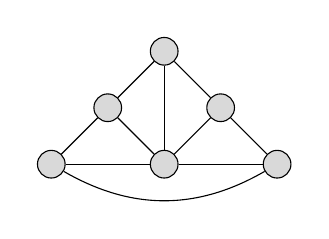
\begin{tikzpicture}
            \matrix[nice graph]{
                          &           & \mknode A &           &           \\
                          & \mknode B &           & \mknode C &           \\
                \mknode D &           & \mknode E &           & \mknode F \\
            } ;

            \graph[use existing nodes]{
                A -- B -- D -- E -- F -- C -- A -- E;
                E -- B ;
                E -- C ;
                D --[bend right=30] F;
            } ;
        \end{tikzpicture}
    \end{center}
    \caption{
        A counterexample showing that a graph having no $K_4$ subgraph cannot
        in general be $3$-colored. The graph shown above has chromatic number
        $4$.
    }
    \label{fig:counterexample}
\end{figure}

\question{Art gallery theorem}

\begin{prop}
    Let $P$ be a polygon in the plane such that at most two angles of $P$
    exceed $180\degrees$. The polygon $P$ can be guarded by two guards.
\end{prop}

\begin{proof}
    By cases.

    \begin{description}
        \item[Case.] There are no obtuse angles in the polygon.

            The polygon is therefore convex. Hence, any vertex in the polygon
            can be joined to every other vertex not adjacent to it with an edge
            not leaving the boundary of the polygon. This means that a guard
            can be placed on any vertex of the polygon and see every wall.

        \item[Case.] There is exactly one obtuse angle.

            We can create an edge from this vertex such that it divides the
            angle in two. This edge will typically intersect another edge,
            where we create another vertex. (So we subdivide the polygon, but
            this does not cause a problem because the angle of this vertex is
            \emph{exactly} $180\degrees$.) This process creates two polygons
            with no $180\degrees$ angles. Hence, we can use the argument from
            the previous case and pick any vertex in those polygons to place a
            guard. By construction, the two polygons share a vertex, so we
            place one guard there to watch the whole art gallery.

        \item[Case.] There is exactly two obtuse angles.

            Let $u, v$ be the vertices with obtuse angles. Apply the
            subdivision procedure of the previous case to split the polygon
            into two polygons. One of these polygons falls under the previous
            case, so it can be watched by one guard. The other polygon is a
            convex polygon, so it can be watched by placing a guard on any
            vertex.
    \end{description}
\end{proof}

Sometimes, two guards are in fact required. Figure $\ref{fig:two-guards}$ shows
an example.

\begin{figure}[ht]
    \begin{center}
        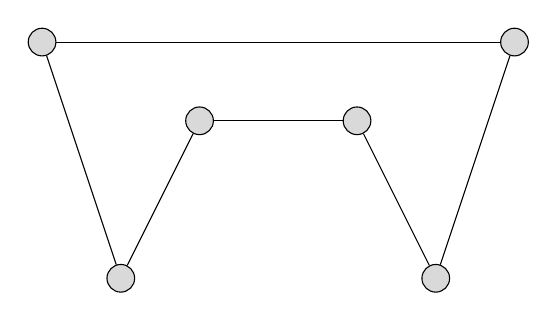
\begin{tikzpicture}
            \node[mynode] at (-3, -0) (A) {} ;
            \node[mynode] at (-1, -1) (B) {} ;
            \node[mynode] at (-2, -3) (C) {} ;
            \node[mynode] at (2, -3) (D) {} ;
            \node[mynode] at (1, -1) (E) {} ;
            \node[mynode] at (3, -0) (F) {} ;

            \graph[use existing nodes]{
                A -- C -- B -- E -- D -- F -- A ;
            } ;
        \end{tikzpicture}
    \end{center}
    \caption{
        The ``tooth graph'' can be guarded by at least two guards, and this
        lower bound is tight.
    }
    \label{fig:two-guards}
\end{figure}

\question{Kuratowski's theorem}

\begin{prop}
    Suppose that $G$ is a non-planar graph and furthermore that $G \setminus e$
    is planar for every edge $e$ of $G$. Then, at most six vertices of $G$ have
    degree three or more.
\end{prop}

\begin{proof}
    Since $G$ is non-planar, it has a subgraph $H \subseteq G$ such that $H$ is
    a subdivision of $K_{3,3}$ or $K_5$. However, if $G \setminus e$ for any
    $e$ is planar, removing more vertices or edges could not result in a
    non-planar graph. Hence, no \emph{proper} subgraph of $G$ is non-planar,
    i.e. $H = G$. The graph $G$ itself is therefore a subdivision of $K_{3, 3}$
    or of $K_5$.

    Suppose $G$ is a subdivision of $K_{3, 3}$. Then, it has in particular the
    six original vertices of $K_{3, 3}$, which each have degree at least three.
    (Subdividing a graph does not decrease the degree of any vertex.) The
    vertices added by the subdivision process always have degree two. Hence, at
    most six vertices in $G$ with degree at least three.

    Suppose $G$ is a subdivision of $K_{5}$. By a similar argument, it has five
    vertices with degree $4$. Any other vertices were added by the subdivision
    process, and hence have degree two. Therefore there are at most six
    vertices in $G$ with degree at least three.
\end{proof}

\question{Testing planarity}

The first graph is non-planar. To see this, contract the edge joining the two
vertices at the top of the graph, and proceed in a clockwise fashion joining
every other pair of vertices. This produces the complete graph on seven
vertices. Deleting two vertices results in $K_5$. Hence, the graph has a $K_5$
minor, and is therefore non-planar.

The secon graph is planar. Figure $\ref{fig:planar}$ shows a planar drawing.

\begin{figure}[ht]
    \begin{center}
        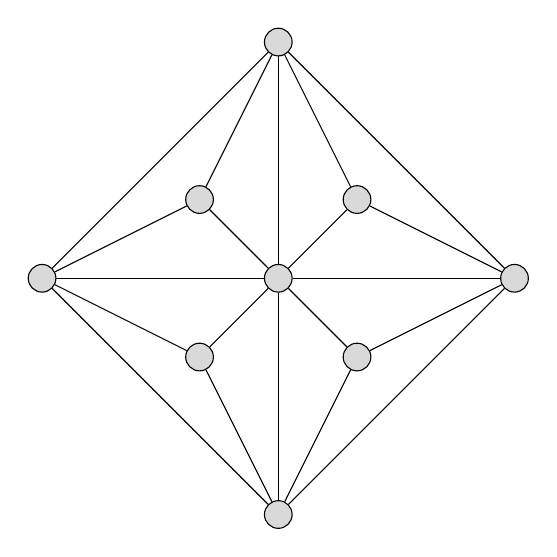
\begin{tikzpicture}
            \node[mynode] at (-3, 0)  (left)         {};
            \node[mynode] at (0, 3)  (top)          {};
            \node[mynode] at (0, -3)   (bottom)       {};
            \node[mynode] at (3, 0)   (right)        {};
            \node[mynode] at (0, 0)   (center)       {};

            \node[mynode] at (-1, -1) (bottomleft)     {};
            \node[mynode] at (1, 1)   (topright)    {};
            \node[mynode] at (1, -1)  (bottomright) {};
            \node[mynode] at (-1, 1)  (topleft)  {};

            \graph[use existing nodes]{
                left -- top -- right -- bottom -- left ;
                left -- center -- top;
                right -- center -- bottom;
                topleft -- { top, left, center } ;
                topright -- { top, right, center } ;
                bottomleft -- { bottom, left, center } ;
                bottomright -- { bottom, right, center } ;
            } ;
        \end{tikzpicture}
    \end{center}
    \caption{
        A planar drawing of the second graph.
    }
    \label{fig:planar}
\end{figure}

\end{document}
